% =====================================================================
%  AI251P Applied Computer Vision -- Capstone Project
%  Phase 2 Report Template (M4, M5, M8, 45 points, due 15 November 2026)
%
%  How to use:
%   * Fill in the team details in the "TEAM DETAILS" block below.
%   * Replace every grey italic prompt (\prompt{...}) with your own text.
%   * Adapt the methods to your problem: the prompts say what must be
%     shown, and the "e.g." hints are examples, not required steps.
%   * Fill every table. Add, remove or rename rows and columns to fit
%     your task, and say why when something does not apply.
%   * Put your figures in the figures/ folder and replace
%     figures/placeholder.png with your own file names.
%   * Every reported figure must state the data split, the input
%     resolution and the thresholds used.
%   * "Optional extras" are not required for full credit.
%   * Teams of 5 must also complete Section 5 (Open-world extension).
%     Teams of 3 or 4 delete Section 5.
% =====================================================================
\documentclass[11pt,a4paper]{article}

\usepackage[T1]{fontenc}
\usepackage[utf8]{inputenc}
\usepackage{mathpazo}
\usepackage[margin=2.2cm]{geometry}
\usepackage{booktabs,tabularx,array,multirow}
\usepackage{graphicx}
\usepackage{caption}
\usepackage{float}
\usepackage{enumitem}
\usepackage{amsmath,amssymb}
\usepackage{xcolor}
\usepackage{fancyhdr}
\usepackage[colorlinks=true,linkcolor=blue!50!black,urlcolor=blue!50!black]{hyperref}

% ---------------------------------------------------------------------
%  TEAM DETAILS -- edit these
% ---------------------------------------------------------------------
\newcommand{\teamname}{Project 5}
\newcommand{\projecttitle}{Automated Triage of Camera-Trap Imagery}

% ---------------------------------------------------------------------
%  Helpers
% ---------------------------------------------------------------------
% Grey italic prompt: delete it and write your own text in its place.
\newcommand{\prompt}[1]{\leavevmode{\color{gray!80!black}\itshape #1}}
% Blank line for short answers
\newcommand{\blank}{\rule{0pt}{2.2ex}}
% Points label in section titles: \pts{teams of 3-4}{teams of 5}
\newcommand{\pts}[2]{\texorpdfstring{\hfill{\normalsize\mdseries(#1 points; teams of 5: #2)}}{}}
\newcommand{\ptsone}[1]{\texorpdfstring{\hfill{\normalsize\mdseries(#1 points)}}{}}
% Heading for optional material
\newcommand{\optextras}{\subsection*{Optional extras {\normalsize\mdseries\itshape(not required for full credit)}}}
% Threshold symbols
\newcommand{\tconf}{$\tau_{\text{conf}}$}
\newcommand{\tnms}{$\tau_{\text{NMS}}$}
% Checklist
\newlist{checklist}{itemize}{1}
\setlist[checklist]{label=$\square$,leftmargin=1.6em,itemsep=2pt}
\newcolumntype{Y}{>{\raggedright\arraybackslash}X}
\renewcommand{\arraystretch}{1.25}
\setlength{\parindent}{0pt}
\setlength{\parskip}{4pt}

\pagestyle{fancy}
\fancyhf{}
\lhead{\itshape AI251P Applied Computer Vision}
\rhead{\itshape Capstone Phase 2 Report -- \teamname}
\cfoot{\thepage}
\setlength{\headheight}{14pt}

\begin{document}

% =====================================================================
\begin{center}
  {\large AI251P Applied Computer Vision}\\[4pt]
  {\LARGE\bfseries Capstone Project -- Phase 2 Report}\\[6pt]
  {\Large \projecttitle}\\[4pt]
  \teamname\ \textperiodcentered\ Phase 2 (M4, M5, M8, 45 points) \textperiodcentered\ Due 15 November 2026
\end{center}
\vspace{4pt}

% =====================================================================
\section{Team and system}

\begin{tabularx}{\linewidth}{@{}l Y@{}}
\toprule
Field & Your answer \\
\midrule
Team name & Project 5 \\
Team size & 4 \\
Topic & Example topic no.\ 5: Automated Triage of Camera-Trap Imagery \\
Code repository and commit hash & \url{https://github.com/salehdev3/Capstone_5/tree/v2} \;\; \texttt{commit pending} \\
W\&B project & \url{https://wandb.ai/saleh-alanazi-ministry-of-interior/camera-trap-phase1} \\
Deployed service / demo & \prompt{URL, or how to run it locally} \\
Model card & \prompt{Link or appendix reference} \\
\bottomrule
\end{tabularx}

\subsection*{Team members}

\begin{tabularx}{\linewidth}{@{}l l l Y@{}}
\toprule
Name & Student ID & Workstream & Phase 2 contribution \\
\midrule
 &  & 2. Detection & Detector training, threshold analysis and error review \\
 &  & 3. Segmentation & Mask verification, fine-tuning and evaluation \\
 &  & 4. Integration & Pipeline, service, ONNX and benchmark \\
 &  & 1. Data and classification & Data provenance and Phase 1 classifier handoff \\
\bottomrule
\end{tabularx}

\smallskip
The four workstreams are assigned to the four team members above.

\subsection*{Points by team size}

\begin{tabularx}{\linewidth}{@{}Y c c@{}}
\toprule
Component & Teams of 3--4 & Teams of 5 \\
\midrule
Object detection (M4) & 15 & 12 \\
Segmentation (M5) & 15 & 12 \\
Integration and deployment (M8) & 15 & 11 \\
Open-world extension (two topics, 5 points each) & -- & 10 \\
\midrule
\textbf{Total} & \textbf{45} & \textbf{45} \\
\bottomrule
\end{tabularx}

\subsection*{System overview}

\begin{figure}[H]
  \centering
  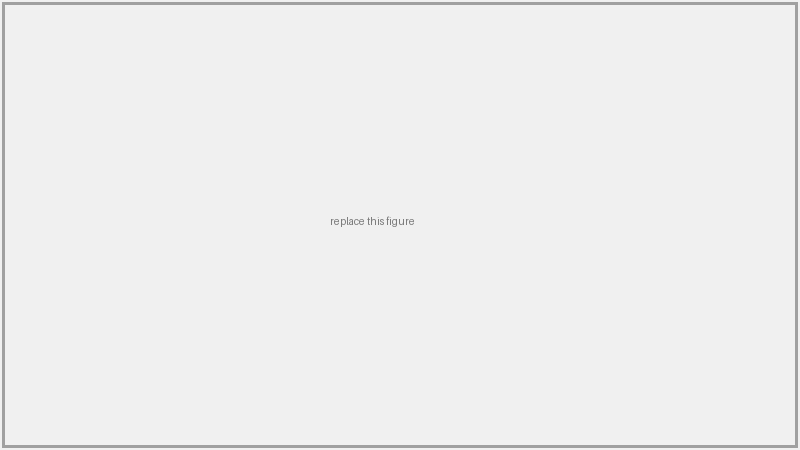
\includegraphics[width=0.9\linewidth]{figures/placeholder.png}
  \caption{End-to-end pipeline, from the input image or video to the output the user receives.}
\end{figure}

{\small
\begin{tabularx}{\linewidth}{@{}l l Y Y Y@{}}
\toprule
Component & Model & Input & Output & Function in the system \\
\midrule
Classifier (Phase 1) & & & & \\
Detector (M4) & & & & \\
Segmentation (M5) & & & & \\
\bottomrule
\end{tabularx}}

\subsection*{Acceptance criteria (fixed in Phase 1)}

\prompt{Copy your Phase 1 criteria unchanged. If you add or change a criterion, mark it and say why. Say how each criterion is checked (ideally by a script) and state the conditions it refers to. Section 4.6 reports the verdict.}

\begin{tabularx}{\linewidth}{@{}Y l l Y@{}}
\toprule
Criterion & Metric & Threshold & Conditions (split, hardware, settings) \\
\midrule
\prompt{e.g.\ critical-class recall} & Recall & $\geq 0.90$ & \prompt{Test split, at the operating point} \\
\prompt{e.g.\ latency} & p95 latency & $\leq 200$\,ms & \prompt{e.g.\ T4 GPU, batch 1, 640\,px, end to end} \\
 & & & \\
\bottomrule
\end{tabularx}

\subsection*{Follow-up on the Phase 1 data-improvement plan}

\begin{tabularx}{\linewidth}{@{}Y l Y@{}}
\toprule
Planned action (Phase 1) & Done? & Measured effect \\
\midrule
 & Yes / No / Partly & \\
 & & \\
\bottomrule
\end{tabularx}

% =====================================================================
\section{Object detection (M4)\pts{15}{12}}

\textbf{Task:} \prompt{The objects detected, the classes, and what the detections are used for in the system.}

\prompt{Choose models, thresholds and settings on the validation split; evaluate the test split once.}

\subsection{Annotation conversion and verification}

\begin{tabularx}{\linewidth}{@{}Y l Y@{}}
\toprule
Item & Count & Notes \\
\midrule
Source format $\rightarrow$ target format & -- & \prompt{e.g.\ VOC XML $\rightarrow$ YOLO txt} \\
Boxes converted & & \\
Boxes fixed (e.g.\ clipped to the image) & & \\
Boxes or objects removed, and why & & \\
Background images (no objects) & & \\
\bottomrule
\end{tabularx}

\medskip
\begin{tabularx}{\linewidth}{@{}l r r Y@{}}
\toprule
Split & Images & Boxes & Boxes per class \\
\midrule
Train & & & \\
Validation & & & \\
Test & & & \\
\bottomrule
\end{tabularx}

\medskip
\textbf{Data checks}

\smallskip
\prompt{The checks you ran on the detection data, what you found and what you did about it. Choose the checks that matter for your data, e.g.\ class balance per split, object sizes at your input resolution, near-duplicates across splits, crowded images, label errors.}

\smallskip
\begin{tabularx}{\linewidth}{@{}l Y Y@{}}
\toprule
Check & Finding & Action \\
\midrule
 & & \\
 & & \\
 & & \\
\bottomrule
\end{tabularx}

\begin{figure}[H]
  \centering
  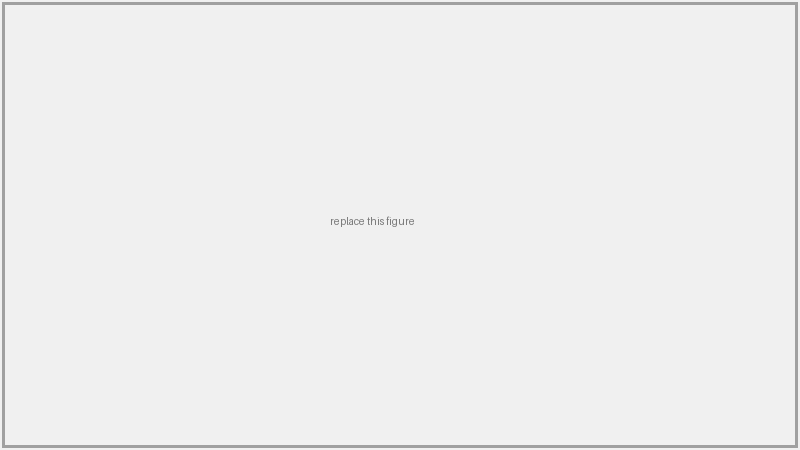
\includegraphics[width=0.9\linewidth]{figures/placeholder.png}
  \caption{Converted boxes drawn back onto sample images to verify the conversion.}
\end{figure}

\subsection{Fine-tuning}

{\small
\begin{tabularx}{\linewidth}{@{}l Y l Y r r@{}}
\toprule
Run (W\&B link) & Model and pretrained weights & Input res. & What changed in this run & Val.\ mAP50 & Val.\ mAP50--95 \\
\midrule
 & & & \prompt{Baseline settings} & & \\
 & & & & & \\
\bottomrule
\end{tabularx}}

\smallskip
\textbf{Selected model and why:} \prompt{One or two sentences. Mention the augmentations you chose and why they suit your data.}

\begin{figure}[H]
  \centering
  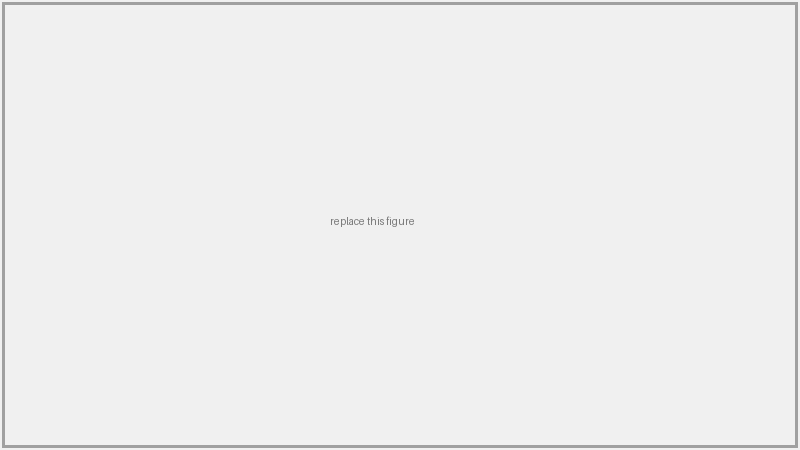
\includegraphics[width=0.9\linewidth]{figures/placeholder.png}
  \caption{Training and validation curves of the selected run. \prompt{Comment on convergence and over-fitting, and how you chose the checkpoint.}}
\end{figure}

\subsection{Threshold sweep and operating point}

\prompt{Sweep the confidence threshold (and the NMS IoU threshold, if your detector uses NMS) on the validation split. Choose the operating point with a rule that fits your application, e.g.\ the best F1, a minimum recall on a critical class, or a minimum precision.}

\begin{tabularx}{\linewidth}{@{}Y Y r r r@{}}
\toprule
\tconf & \tnms\ (if used) & Precision & Recall & F1 \\
\midrule
 & & & & \\
 & & & & \\
 & & & & \\
\midrule
\textbf{Selected:} & & & & \\
\bottomrule
\end{tabularx}

\begin{figure}[H]
  \centering
  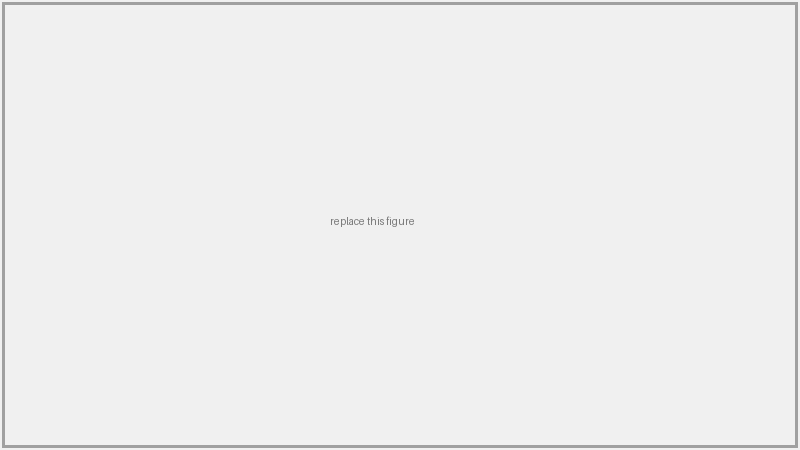
\includegraphics[width=0.6\linewidth]{figures/placeholder.png}
  \caption{Precision, recall and F1 against \tconf\ on the validation split.}
\end{figure}

\textbf{Justification of the operating point:} \prompt{Why this rule and threshold suit the cost of false positives and false negatives in your application.}

\subsection{Test results}

\prompt{Measure mAP at a low confidence threshold (not at the deployment threshold), and precision, recall and F1 at the selected operating point. State the thresholds used.}

{\small
\begin{tabularx}{\linewidth}{@{}Y r r r r r r@{}}
\toprule
Class & Instances & AP50 & AP50--95 & P @ op. & R @ op. & F1 @ op. \\
\midrule
 & & & & & & \\
 & & & & & & \\
\midrule
\textbf{All classes} & & & & & & \\
\bottomrule
\end{tabularx}}

\smallskip
\textbf{Weak classes:} \prompt{Why each weak class is weak (too few examples, confusable classes, label problems) and what would help.}

\medskip
\prompt{Recall by object size. State how you define the size bins (e.g.\ COCO bins on the box area at your input resolution).}

\begin{tabularx}{\linewidth}{@{}Y r r@{}}
\toprule
Object size & Instances & Recall @ op. \\
\midrule
Small & & \\
Medium & & \\
Large & & \\
\bottomrule
\end{tabularx}

\subsection{Error analysis}

\prompt{Test split, at the operating point. Rename, add or merge types to fit your problem, and say how each type is defined.}

\begin{tabularx}{\linewidth}{@{}l Y r r@{}}
\toprule
Type & Definition & Count & Share (\%) \\
\midrule
Duplicate & \prompt{e.g.\ a second box on an object already detected} & & \\
Classification & \prompt{e.g.\ right place, wrong class} & & \\
Localisation & \prompt{e.g.\ right class, box too loose or too tight} & & \\
Background & \prompt{e.g.\ no object there} & & \\
\midrule
Missed (FN) & \prompt{Object with no matching detection} & & -- \\
\bottomrule
\end{tabularx}

\begin{figure}[H]
  \centering
  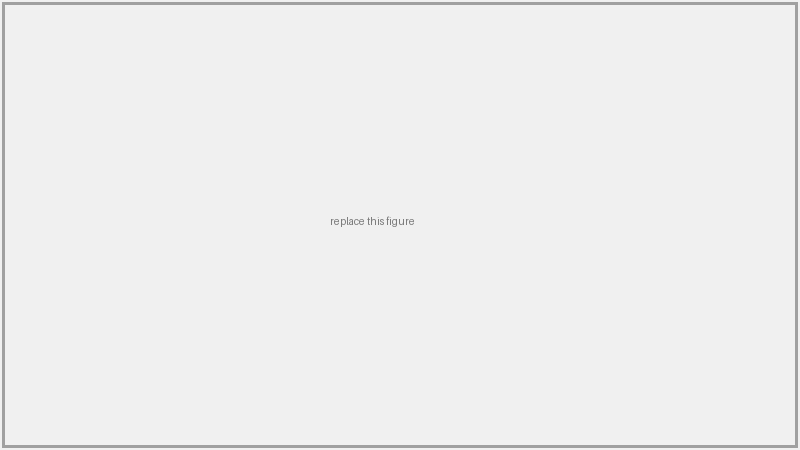
\includegraphics[width=0.48\linewidth]{figures/placeholder.png}\hfill
  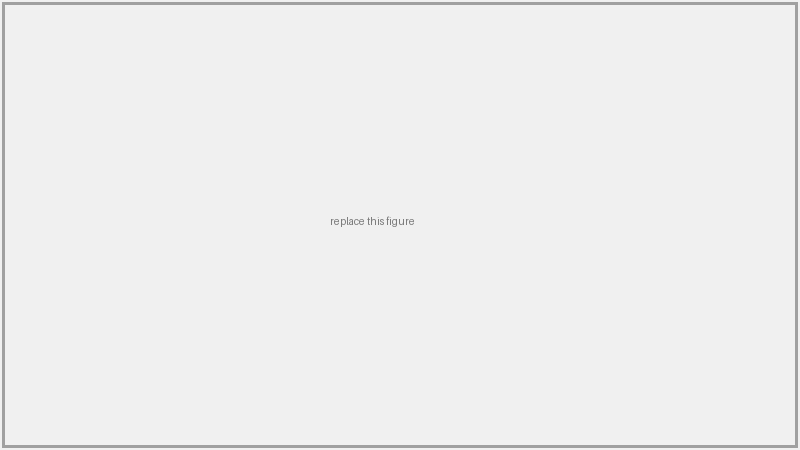
\includegraphics[width=0.48\linewidth]{figures/placeholder.png}
  \caption{(Left) false positives; (right) false negatives, at the operating point on the test set.}
\end{figure}

\textbf{Main causes of false negatives:} \prompt{e.g.\ small objects, occlusion, poor lighting.}

\textbf{Failure case:} \prompt{One image: what the detector did, why it failed, and what would fix it.}

\textbf{Next fix:} \prompt{The largest source of errors and the change you would make for it.}

\subsection{Inference on images and video}

\prompt{Run the detector on test images and on a video clip at the operating point. Report the speed (FPS), the hardware and the input resolution.}

\optextras

\begin{itemize}[leftmargin=1.2em,itemsep=1pt]
  \item Calibration of the confidence scores (reliability diagram, ECE).
  \item AP against the IoU threshold, to separate loosely boxed objects from missed ones.
  \item Robustness to conditions your data may meet (blur, low light, compression, weather).
  \item Confidence intervals for mAP (e.g.\ bootstrap).
  \item Remedies for small objects (higher resolution, tiled inference), or a comparison with another detector family.
  \item Tracking across video frames.
\end{itemize}

% =====================================================================
\section{Segmentation (M5)\pts{15}{12}}

\textbf{Task:} \prompt{Semantic or instance segmentation, the classes, and what the masks are used for in the system (e.g.\ area, count, share of shelf). Explain why this type of segmentation fits your problem.}

\prompt{Choose the model, thresholds and post-processing on validation; evaluate the test split once.}

\subsection{Ground-truth masks}

\begin{tabularx}{\linewidth}{@{}l Y@{}}
\toprule
Item & Your answer \\
\midrule
Source of masks & \prompt{e.g.\ dataset masks, SAM prompted with boxes or points, manual} \\
Images with masks (train / val / test) & \\
Class distribution & \prompt{e.g.\ pixel share or number of objects per class} \\
How masks were checked & \prompt{Automatic checks (e.g.\ valid label values, mask size) and visual checks: how many, by whom} \\
Masks corrected or rejected & \\
Label format & \prompt{e.g.\ index maps, COCO polygons, RLE; how unlabelled regions are handled} \\
\bottomrule
\end{tabularx}

\begin{figure}[H]
  \centering
  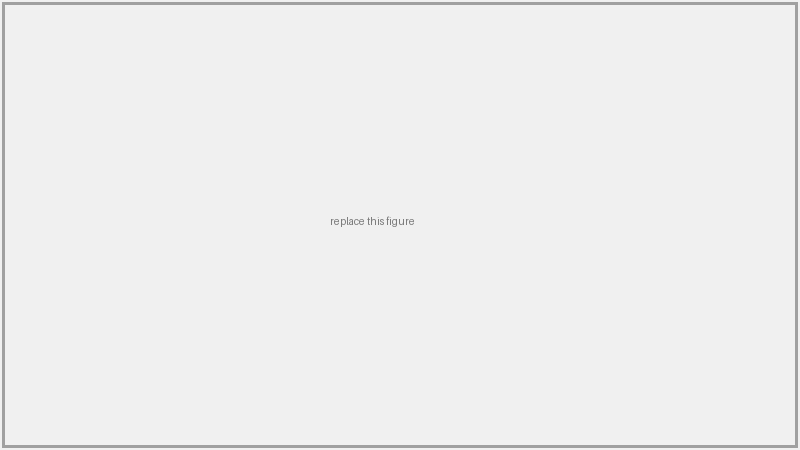
\includegraphics[width=0.9\linewidth]{figures/placeholder.png}
  \caption{Sample ground-truth masks overlaid on the images.}
\end{figure}

\subsection{Model and training}

\prompt{Compare the fine-tuned model with a baseline that shows what fine-tuning adds (e.g.\ the model before fine-tuning, a pretrained model used as is, or a simple method). Say what you changed between runs and why.}

{\small
\begin{tabularx}{\linewidth}{@{}l Y l Y l r@{}}
\toprule
Run (W\&B) & Model and initial weights & Train / eval res. & Training setup (loss, augmentation, optimiser) & Epochs / iter. & Val.\ metric \\
\midrule
Baseline & & & & & \\
 & & & & & \\
 & & & & & \\
\bottomrule
\end{tabularx}}

\smallskip
\textbf{Selected run and why (chosen on validation):} \prompt{One or two sentences.}

\begin{figure}[H]
  \centering
  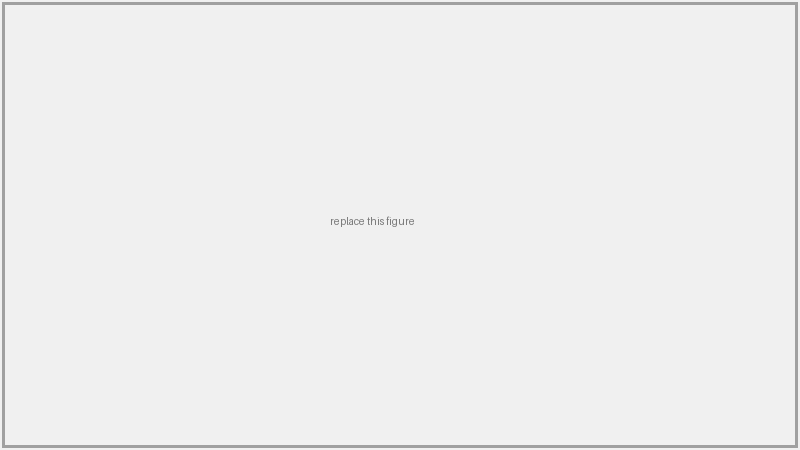
\includegraphics[width=0.9\linewidth]{figures/placeholder.png}
  \caption{Training loss and validation metric. \prompt{Comment on convergence and how you chose the checkpoint.}}
\end{figure}

\subsection{Thresholds and post-processing}

\prompt{If your output depends on thresholds or post-processing (e.g.\ confidence, mask threshold, morphological operations, minimum area), choose them on validation and report them here. Otherwise, say so.}

\begin{tabularx}{\linewidth}{@{}l Y l l@{}}
\toprule
Setting & Values tried & Validation metric & Chosen \\
\midrule
 & & & \\
 & & & \\
\bottomrule
\end{tabularx}

\subsection{Test results}

\prompt{Report the metrics that apply to your task (mask mAP50--95 for instance segmentation; mean IoU and Dice for semantic segmentation), plus any others your application needs. Say how each metric is computed (e.g.\ how unlabelled pixels are handled and how classes are averaged).}

{\small
\begin{tabularx}{\linewidth}{@{}Y l r r r r@{}}
\toprule
Model & Split & Mask mAP50--95 & mIoU & Mean Dice & Other \\
\midrule
Baseline & Val & & & & \\
Selected run & Val & & & & \\
Selected run & Test & & & & \\
\bottomrule
\end{tabularx}}

\medskip
\begin{tabularx}{\linewidth}{@{}Y r r r@{}}
\toprule
Class & IoU & Dice & Mask AP \\
\midrule
 & & & \\
 & & & \\
\bottomrule
\end{tabularx}

\smallskip
\textbf{Application measure:} \prompt{The quantity the masks give the user, on the test split, e.g.\ count error, area error, or agreement on a yes/no decision.}

\subsection{Error analysis}

\begin{figure}[H]
  \centering
  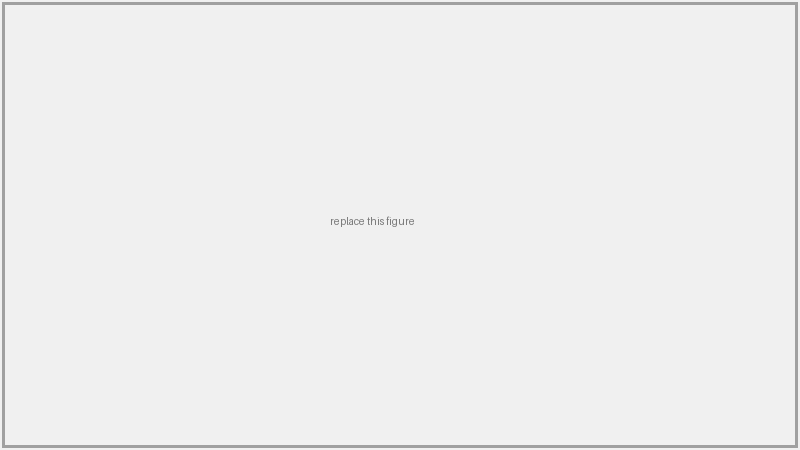
\includegraphics[width=0.9\linewidth]{figures/placeholder.png}
  \caption{Predictions vs.\ ground truth on test images, including failures. \prompt{Semantic segmentation: a confusion matrix also helps.}}
\end{figure}

\begin{tabularx}{\linewidth}{@{}Y r Y@{}}
\toprule
Error pattern & Examples & Likely cause \\
\midrule
 & & \\
 & & \\
\bottomrule
\end{tabularx}

\textbf{Failure case:} \prompt{One image: what the model did, why it failed, and what would fix it.}

\optextras

\begin{itemize}[leftmargin=1.2em,itemsep=1pt]
  \item Results by object size or by class group; the effect of input resolution.
  \item SAM (or another promptable model) compared with your trained model on the same prompts.
  \item Merging classes that are easily confused, and the effect on the metrics.
\end{itemize}

% =====================================================================
\section{System integration and deployment (M8)\pts{15}{11}}

\prompt{Measure on the hardware you deploy on, through the path you deploy, and state the conditions of every number.}

\subsection{End-to-end pipeline}

\prompt{Time each stage per input. Add or rename stages to match your pipeline. Measure the end-to-end time directly rather than adding up the stages.}

\begin{tabularx}{\linewidth}{@{}l Y r r@{}}
\toprule
Stage & Implementation & p50 (ms) & p95 (ms) \\
\midrule
Pre-processing & & & \\
Model inference: \prompt{model 1} & & & \\
Model inference: \prompt{model 2} & & & \\
Post-processing and decision & & & \\
\midrule
\textbf{End to end} & & & \\
\bottomrule
\end{tabularx}

\smallskip
\textbf{Conditions:} \prompt{Hardware, runtime, input size, number of warm-up and timed inputs.}

\subsection{Release and manifest}

\prompt{What the release contains and how the service uses it. The service should read its settings from the manifest rather than from values typed into the code.}

\begin{tabularx}{\linewidth}{@{}l Y@{}}
\toprule
Item & Your answer \\
\midrule
Model file(s) and checksum & \\
Class names and order & \\
Input size and pre-processing & \\
Thresholds & \\
Library and runtime versions & \\
Manifest link & \\
\bottomrule
\end{tabularx}

\subsection{Input and output contracts}

\begin{tabularx}{\linewidth}{@{}l Y@{}}
\toprule
Contract & Your answer \\
\midrule
Input & \prompt{Format, colour order, resolution, resizing or letterboxing, normalisation, batch size} \\
Output & \prompt{Fields, units, coordinate system, and the decision returned to the user} \\
Thresholds served & \prompt{The operating-point thresholds used by the service} \\
Invalid input & \prompt{What the service does with a wrong size, a corrupt image or an empty frame} \\
\bottomrule
\end{tabularx}

\subsection{ONNX export and parity}

\textbf{Export settings:} \prompt{Opset, fixed or dynamic input shapes, and what is inside the exported model vs.\ in your code.}

\begin{tabularx}{\linewidth}{@{}Y l l l@{}}
\toprule
Check (PyTorch vs.\ ONNX) & Tolerance & Result & Pass? \\
\midrule
Difference in raw outputs (e.g.\ scores, boxes) & & & \\
Same decisions at the operating point (e.g.\ \% of detections matched) & & & \\
Same metric on the evaluation set & & & \\
Reduced precision (FP16 / INT8), if used & & & \\
\bottomrule
\end{tabularx}

\subsection{HTTP service}

\begin{tabularx}{\linewidth}{@{}l Y@{}}
\toprule
Item & Your answer \\
\midrule
Framework and hosting & \prompt{e.g.\ FastAPI, Modal, Gradio} \\
Endpoint(s) & \\
Hardware & \\
Checks at start-up & \prompt{e.g.\ model file verified, expected device available, a test input gives the expected output} \\
Example request & \texttt{curl -X POST -F "file=@img.jpg" https://.../predict} \\
\bottomrule
\end{tabularx}

\begin{figure}[H]
  \centering
  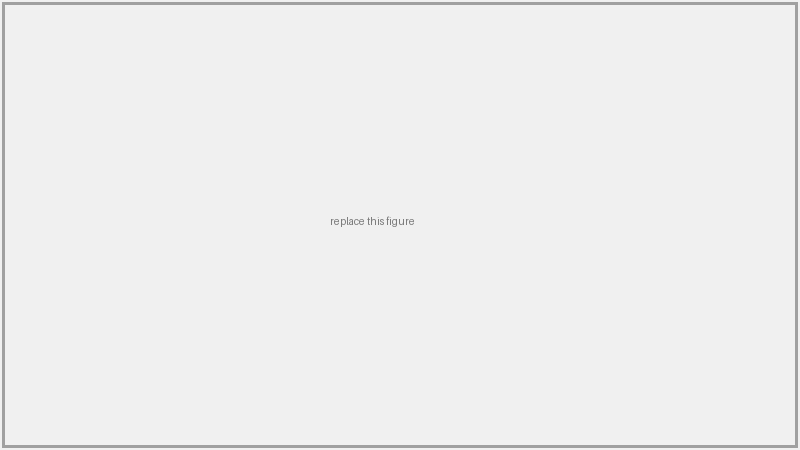
\includegraphics[width=0.7\linewidth]{figures/placeholder.png}
  \caption{The running service: a request and its response.}
\end{figure}

\subsection{Benchmark}

\textbf{Conditions:} \prompt{Device, runtime versions, input resolution, batch size, warm-up, number of timed calls (enough for the percentiles you report), what the time includes, and how memory was measured.}

{\small
\begin{tabularx}{\linewidth}{@{}Y l r r r r r r@{}}
\toprule
Backend & Precision & Batch & p50 (ms) & p95 (ms) & p99 (ms) & Throughput (img/s) & Memory (MB) \\
\midrule
\prompt{e.g.\ PyTorch} & & & & & & & \\
\prompt{e.g.\ ONNX Runtime} & & & & & & & \\
 & & & & & & & \\
\bottomrule
\end{tabularx}}

\begin{figure}[H]
  \centering
  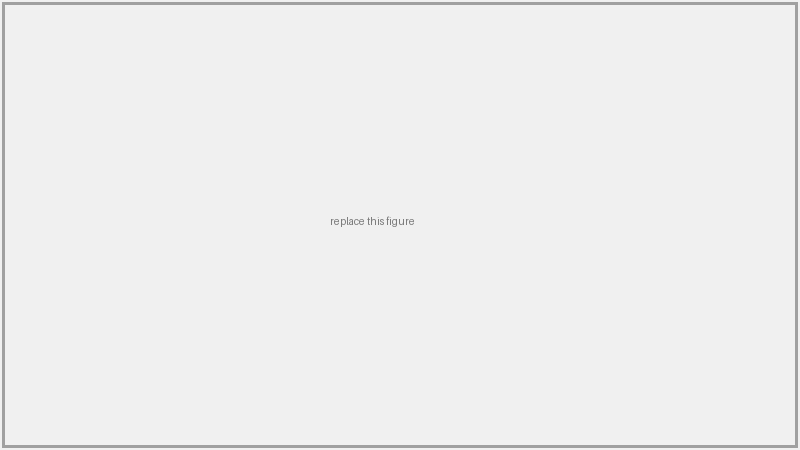
\includegraphics[width=0.6\linewidth]{figures/placeholder.png}
  \caption{\prompt{A benchmark figure that suits your deployment, e.g.\ latency and throughput against batch size, or the latency distribution per backend.}}
\end{figure}

\subsection{Verdict against the acceptance criteria}

\begin{tabularx}{\linewidth}{@{}Y l l l@{}}
\toprule
Criterion & Threshold & Measured & Pass / Fail \\
\midrule
 & & & \\
 & & & \\
\midrule
\multicolumn{3}{@{}l}{\textbf{Preliminary decision}} & \textbf{GO / NO-GO} \\
\bottomrule
\end{tabularx}

\smallskip
\textbf{For each FAIL:} \prompt{Why it failed, and what change would fix it at what cost.}

\prompt{The final decision, the failure gallery and the model card are presented in the final presentation. Summarise the main failure modes and the out-of-scope uses listed in your model card.}

\optextras

\begin{itemize}[leftmargin=1.2em,itemsep=1pt]
  \item Behaviour when the input source fails (e.g.\ a camera goes offline).
  \item Start-up time, and the first request vs.\ warm requests.
  \item Behaviour under load (queueing, timeouts, scaling).
  \item Quantisation (FP16 / INT8) with its effect on accuracy and speed.
  \item A model card generated from the manifest.
\end{itemize}

% =====================================================================
\section{Obstacles and how they were addressed}

\prompt{List the main obstacles you faced (data, compute, tools, annotation, team coordination, \dots), what they affected, and what you did about them. Write ``None'' if there were none.}

\medskip
{\small
\begin{tabularx}{\linewidth}{@{}Y l Y Y l@{}}
\toprule
Obstacle & Module & Impact on the work & Action taken & Status \\
\midrule
\prompt{e.g.\ ONNX export failed on the segmentation head} & M8 & \prompt{Could not serve masks from ONNX} & \prompt{Exported the detector only; masks served from PyTorch} & Workaround \\
 & & & & \\
 & & & & \\
\bottomrule
\end{tabularx}}

\smallskip
\textbf{Support needed before the final presentation (optional):} \prompt{Anything the instructors can help with.}

% =====================================================================
\section{Submission checklist}

\begin{checklist}
  \item Annotations converted and verified visually; data checks reported
  \item Detector fine-tuned; thresholds swept on validation; operating point justified
  \item mAP50, mAP50--95 and per-class AP on the test split; P/R/F1 at the operating point; recall by object size
  \item False-positive breakdown, FP/FN galleries and at least one detection failure case
  \item Detector run on images and video at the operating point
  \item Ground-truth masks checked; segmentation model fine-tuned and compared with a baseline
  \item Segmentation evaluated with the metrics that apply (mask mAP50--95, mIoU, Dice) and one failure case
  \item End-to-end pipeline with per-stage timing and a manifest
  \item ONNX export with a parity check
  \item Working HTTP service with input and output contracts
  \item p50/p95/p99 latency, throughput and memory measured with warm-up and stated conditions
  \item Verdict reported against the acceptance criteria fixed in Phase 1
  \item Teams of 5: two different open-world topics, each with a function in the system, a baseline and a failure case
  \item Every figure states split, input resolution and thresholds
  \item No data or personal information committed to the repository
\end{checklist}

% =====================================================================
\section{Self-assessment}

{\small
\begin{tabularx}{\linewidth}{@{}l c c c Y Y@{}}
\toprule
Criterion & Teams of 3--4 & Teams of 5 & Self-score & Strongest evidence (section) & Known gap \\
\midrule
Object detection (M4) & 15 & 12 & & & \\
Segmentation (M5) & 15 & 12 & & & \\
Integration and deployment (M8) & 15 & 11 & & & \\
Open-world topic A & -- & 5 & & & \\
Open-world topic B & -- & 5 & & & \\
\midrule
\textbf{Total} & \textbf{45} & \textbf{45} & & & \\
\bottomrule
\end{tabularx}}

\end{document}
